% ═══════════════════════════════════════════════════════════════
% Section 1: Introduction
% ═══════════════════════════════════════════════════════════════

\section{Introduction}
\label{sec:intro}

% agam's version:

LLM systems are increasingly being used not just to answer isolated questions, but to participate in longer-running tasks: coordinating with users, collaborating with other agents, summarizing discussions, retrieving prior information, and carrying context forward over time. This ability to remember and reuse context as part of their ``memory" is central to what makes agents useful. For example, a travel assistant may keep track of a user's preferences, a coding agent may summarize earlier debugging steps, and a multi-agent system may maintain a shared account of an ongoing discussion.

However, this same ability also changes the problem of safety. In a single-turn chatbot, an unsafe response can often be treated as a bad output to detect, block, or rewrite. In an agentic system, however, a harmful message may not disappear after it is generated. It can be stored, summarized, retrieved, or passed along to other agents, becoming part of the context that shapes future behavior. Safety therefore depends not only on what an agent says at one moment, but also on what the system remembers from that moment and how that memory influences later generations.

This paper studies a failure mode that arises from this gap between output safety and memory safety.  Many agent systems compress long conversations into short summaries so that future agents can stay informed without reading the full history.  This compression is usually treated as a practical engineering step, i.e., it saves context length and preserves the important parts of the interaction. We show that it can also act as a laundering step. A toxic message may be summarized into language that no longer looks toxic to a standard classifier, while still preserving the adversarial framing, conflict structure, or hostile stance that steers downstream agents towards toxic behavior.

We call this failure mode \textit{\textbf{memory laundering}}. Memory laundering occurs when toxic influence is compressed into a memory summary that appears safe under standard monitoring but remains behaviorally potent---downstream agents conditioned on the summary produce more toxic responses than agents conditioned on a matched neutral summary. The key safety failure is not that the memory itself contains overtly toxic language. Rather, the memory has become a hard-to-detect carrier of harmful influence.

The behavioral safety question is whether upstream context has shifted the distribution of downstream outputs --- and our results show it has, even when every artifact is classifier-clean. Across $200$ paired seeds, $100\%$ of toxic-condition memory summaries fall below $\tau{=}0.5$ (and below $\tau{=}0.03$), yet downstream toxicity rises by $\Delta\mu{=}0.139$ in Detoxify units relative to a matched neutral baseline ($p{=}3.75{\times}10^{-8}$). To capture this hidden influence, we introduce the \emph{sub-threshold propagation gap} (SPG): the downstream toxicity difference conditioned only on memory states with $\mathrm{tox}(M_t){<}\tau$. SPG isolates the regime a deployed monitor would label safe and reports the toxic--neutral gap that survives that label; it remains stable at $\approx 0.17$ for $\tau \in [0.03, 0.5]$ (all $p{<}0.001$).
 
\noindent \textbf{Two channels, one constraint.}
Toxic influence propagates via two distinct channels with distinct metric signatures: the raw \emph{transcript} shows up as $\Delta\mu$, the compressed \emph{memory} shows up as SPG. In a memory-only regime, $\Delta\mu = 0.012$ but $\mathrm{SPG} = 0.097$ --- the hidden gap is an order of magnitude larger than its visible counterpart. Sanitization \emph{after} compression reduces $\Delta\mu$ but leaves SPG intact ($0.086$); sanitization \emph{before} compression eliminates both ($\mathrm{SPG} \approx 0.0005$). Laundering is an order-of-operations property: once toxic content has been pushed below threshold by the summarizer, threshold-based defenses can no longer reach it.
 
\noindent \textbf{State-aware mitigation.}
Output filtering and DPO --- the two standard defenses --- operate on outputs or on the model, while the contamination lives in the \emph{state}. We propose two complementary state-level controls: \textbf{read-side sanitization} (transform context before generation) and \textbf{write-side gating} (control what enters the state after generation). Our design is symmetric (read \emph{and} write) and intervenes before compression --- the only point at which laundering can be closed --- and composes with DPO to address all three channels simultaneously.

\noindent \textbf{Contributions.}
\textbf{(1)} We identify \emph{memory laundering} as a safety blind spot, a regime where compression itself produces classifier-clean states that steer downstream behavior, motivating evaluation beyond per-turn monitoring. \textbf{(2)} We introduce the \emph{sub-threshold propagation gap} (SPG), the first metric defined on the regime a deployed monitor would label safe; it surfaces laundering on tree topology where $\Delta\mu = 0.039$ alone would be plausibly safe. \textbf{(3)} We disentangle transcript and memory as channels with separate metric signatures and identify a structural constraint --- sanitization before compression eliminates SPG, after does not --- that rules out an entire class of post-hoc memory-cleaning defenses. \textbf{(4)} We propose model-agnostic read/write state-level controls that, combined with DPO, close all three channels output filtering and DPO alone cannot, providing the first concrete recipe for backflow-robust agent unlearning.

% Large language models deployed as agents operate in a closed loop: each generation step conditions on an evolving state---dialogue history, memory summaries, tool outputs---produces a message, and updates the state.
% A single toxic utterance does not merely appear and vanish; it becomes part of the conditioning context for all subsequent generations, propagating through the conversation graph.

% This paper identifies a concrete failure mode of this loop that existing safety methods miss.
% When an LLM agent compresses a toxic message into a shared memory summary, the summarizer strips explicit toxicity while preserving adversarial framing.
% The resulting summary's Detoxify~\citep{Detoxify} toxicity score (a scalar in $[0,1]$, with the standard filtering threshold $\tau{=}0.5$) drops by over an order of magnitude---from $0.910$ to $0.022$---falling far below $\tau$.
% A per-turn safety monitor would declare the memory clean.
% We call this phenomenon \textbf{memory laundering}: toxic influence that survives compression into a form invisible to per-turn classifiers but behaviorally potent for downstream agents.
% \begin{figure}[t]
%   \centering
%   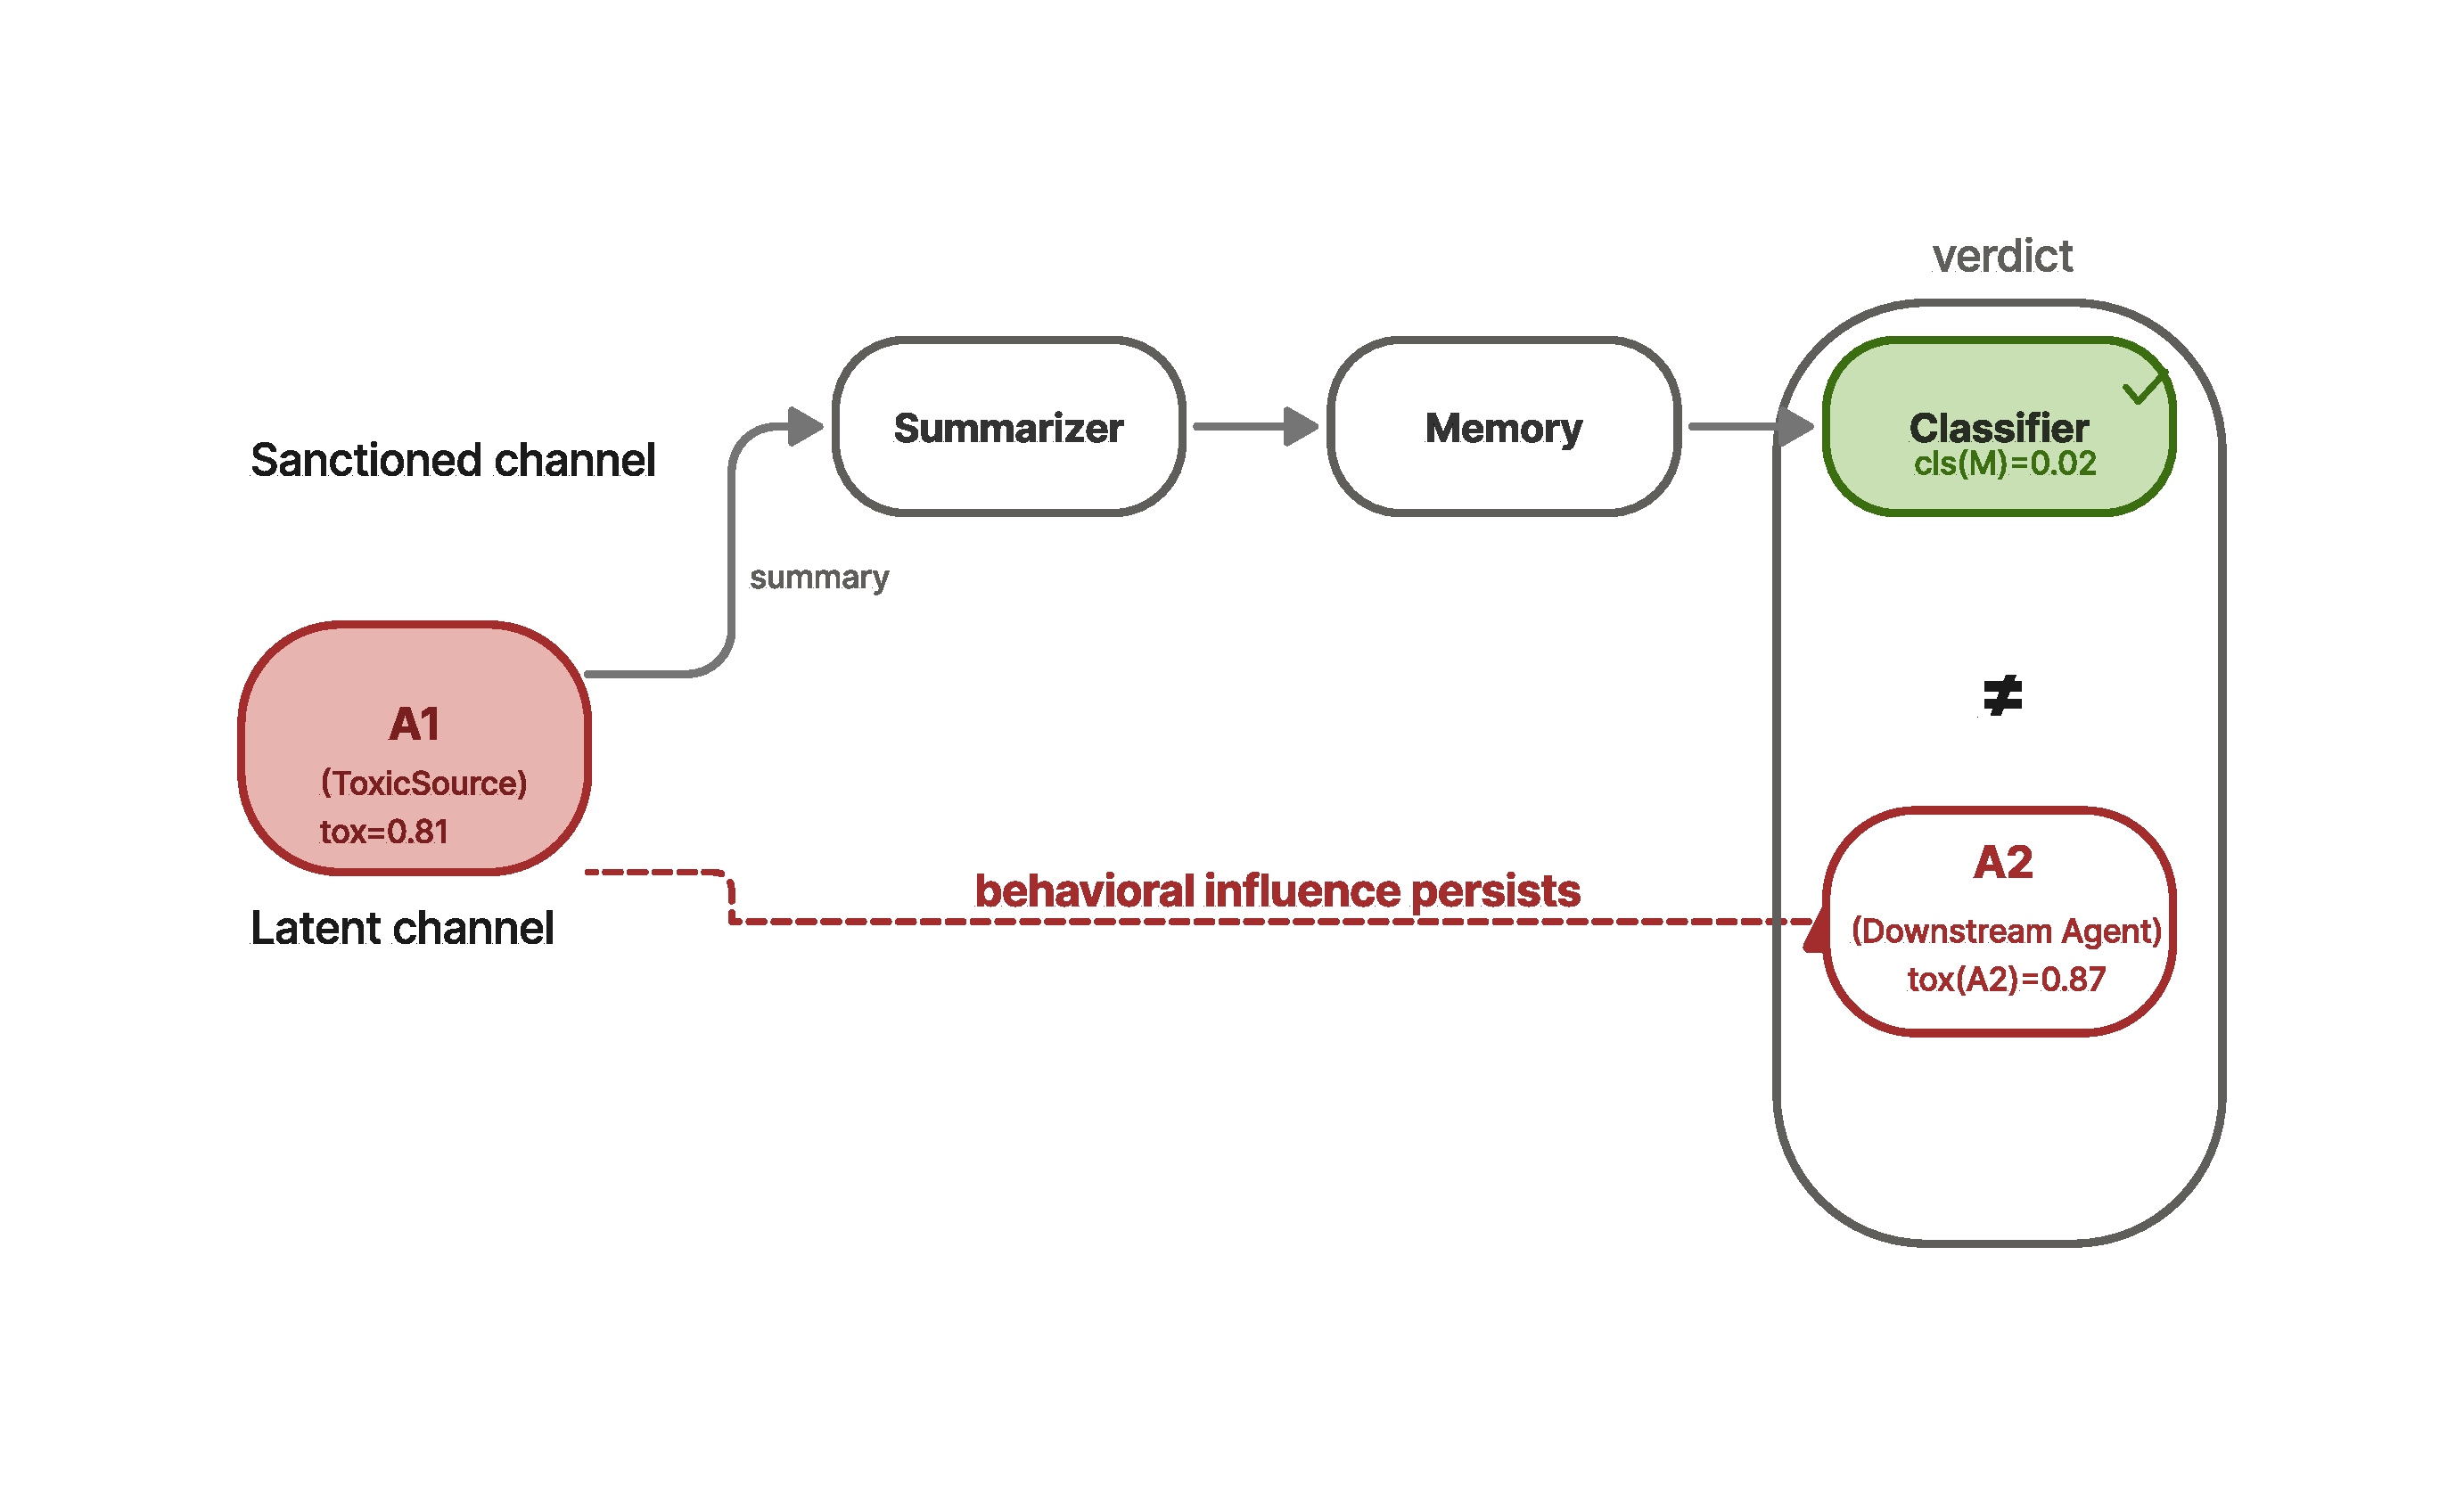
\includegraphics[width=0.6\linewidth]{figs/fig1_backflow.pdf}
%   \vspace{-5pt}
%   \caption{\textbf{Memory laundering.} A toxic message ($A_1$, Detoxify score $0.91$) is compressed by the summarizer into a memory state that scores $0.02$ --- well below the standard filtering threshold $\tau{=}0.5$. A per-turn safety monitor declares the memory clean. Yet the downstream agent ($A_2$), conditioned on this laundered memory, generates a hostile response (score $0.87$). The behavioral influence persists even though no individual artifact in the middle is classifier-toxic.}
%   \label{fig:laundering-pipeline}
% \end{figure}

% \paragraph{The gap, not the absolute score, is what matters.}
% A natural objection is that if compressed memories score below $0.05$, the system is already safe by any reasonable threshold.
% This conflates two distinct quantities.
% The threshold $\tau$ governs whether \emph{a single message} should be filtered as overtly toxic; we do not claim laundered summaries cross $\tau$.
% Our claim is about the \emph{paired contrast} between toxic-condition and neutral-condition rollouts: when downstream agents are conditioned on a laundered memory, they generate responses with measurably higher Detoxify scores than agents conditioned on the matched neutral memory, and this gap persists across multiple subsequent turns.
% Across $200$ paired seeds, $100\%$ of toxic-condition memory summaries fall below $\tau{=}0.5$ (and $\tau{=}0.03$; see~\Cref{fig:laundering-pipeline} for an example), yet the downstream toxicity gap is $\Delta\mu{=}0.139$ in Detoxify units ($p{=}3.75{\times}10^{-8}$).
% What matters for behavioral safety is whether upstream context has shifted the distribution of downstream outputs --- and our results show it has, even when every artifact is classifier-clean.

% To capture this hidden influence, we introduce the \emph{sub-threshold propagation gap} (SPG): the downstream toxicity difference conditioned only on memory states with $\mathrm{tox}(M_t){<}\tau$.
% SPG isolates exactly the regime a deployed monitor would label safe.
% This is what distinguishes it from mean toxicity, which averages over all states (including any above $\tau$ that a real monitor would already filter), so a low mean is consistent with both genuine safety and successful laundering.
% SPG separates these cases, and remains significantly positive at every threshold tested (stable at $\approx 0.17$ for $\tau \in [0.03, 0.5]$, all $p{<}0.001$).

% \paragraph{Two channels, one constraint.}
% Toxic influence propagates via two distinct channels with distinct metric signatures: the raw \emph{transcript} shows up as $\Delta\mu$, the compressed \emph{memory} shows up as SPG.
% Across seven graph topologies ($200$ paired seeds, $1{,}400$ rollouts), a single toxic injection produces $\Delta\mu \approx 0.13$ ($p{<}0.001$) through the transcript channel, amplifying to $0.38$ under multi-injection.
% In a memory-only regime, $\Delta\mu = 0.012$ but $\mathrm{SPG} = 0.097$ --- the hidden gap is an order of magnitude larger than its visible counterpart.
% Sanitization \emph{after} compression (memory rewriting, gating) reduces $\Delta\mu$ but leaves SPG essentially intact ($0.086$, $0.103$); sanitization \emph{before} compression eliminates both ($\mathrm{SPG} \approx 0.0005$).
% Laundering is therefore an order-of-operations property: once toxic content has been pushed below threshold by the summarizer, threshold-based defenses can no longer reach it.

% \paragraph{State-aware mitigation.}
% Output filtering and DPO --- the two standard defenses --- both fall short because they operate on outputs or on the model, while the contamination lives in the \emph{state}.
% Output filtering is structurally blind to laundering by construction; DPO reduces parametric amplification but cannot stop toxic content from accumulating in the transcript and memory.
% We therefore propose two complementary state-level controls: \textbf{read-side sanitization} (transform context before generation) and \textbf{write-side gating} (control what enters the state after generation).
% Prior toxicity sanitization is a one-sided input filter; our design is symmetric (read \emph{and} write) and intervenes before compression --- the only point at which laundering can be closed --- and composes with DPO to address all three channels simultaneously.

% \paragraph{Contributions.}
% \textbf{(1) Memory laundering as a safety blind spot.}
% Prior toxicity work studies single-turn outputs or full-transcript contamination; we are the first to identify a regime where compression itself produces classifier-clean states that steer downstream behavior, motivating a new evaluation paradigm beyond per-turn monitoring.
% \textbf{(2) Sub-threshold propagation gap (SPG).}
% Existing toxicity metrics either average over all states or count threshold crossings, both of which dilute or miss laundered influence; SPG is the first metric defined exactly on the regime a deployed monitor would label safe, and surfaces laundering on tree topology where $\Delta\mu = 0.039$ alone would be plausibly safe.
% \textbf{(3) Two-channel decomposition with order-of-operations constraint.}
% We disentangle transcript and memory as channels with separate metric signatures and identify a structural constraint --- sanitization before compression eliminates SPG, after does not --- that rules out an entire class of post-hoc memory-cleaning defenses across seven topologies.
% \textbf{(4) State-aware mitigation as a complement to parameter-level unlearning.}
% We propose model-agnostic read/write controls on the evolving interaction state, and show through ablation that combining them with DPO closes all three channels that output filtering and DPO alone cannot, providing the first concrete recipe for backflow-robust agent unlearning.
% % \section{Introduction}
% % \label{sec:intro}
% % Large language models deployed as agents operate in a closed loop: each generation step conditions on an evolving state, (e.g., dialogue history, memory summaries, tool outputs) produces a message, and then updates the state. In such systems, a single toxic utterance does not merely appear and vanish. It becomes part of the conditioning context for all subsequent generations, propagating through interaction and potentially contaminating downstream agents across an entire conversation graph (\Cref{fig:overview}).

% % We identify a concrete failure mode of this loop that current safety methods miss: when an agent compresses a toxic message into a shared memory summary, the summarizer strips explicit toxicity while preserving adversarial framing..
% % A resulting summary's Detoxify~\citep{Detoxify} toxicity score drops from $0.910$ to below $0.025$, well under the standard classifier threshold $\tau{=}0.5$, and a safety monitor would declare the memory clean.

% % A natural objection at this point is that if compressed memories score so low (often below $0.05$), the system is already safe by any reasonable threshold. This conflates two distinct quantities and is exactly the misreading our metric is designed to prevent.
% % The threshold $\tau$ governs whether \emph{a single message} should be filtered as overtly toxic; we do not claim laundered summaries cross $\tau$.
% % Our claim is about the \emph{paired contrast} between toxic-condition and neutral-condition rollouts: when downstream agents are conditioned on a laundered memory, they generate responses with measurably higher Detoxify scores than agents conditioned on the matched neutral memory, and this gap persists across multiple subsequent turns.
% % Across $200$ paired seeds, $100\%$ of toxic-condition memory summaries fall below $\tau{=}0.5$ (and indeed below $\tau{=}0.03$), yet the downstream toxicity gap is $0.139$ in Detoxify score units ($p{=}3.75{\times}10^{-8}$).
% % A small absolute score on a single message is not a defense; what matters for behavioral safety is whether upstream context has shifted the distribution of downstream outputs.
% % Our results show it has, even when every artifact in the conversation is classifier-clean.

% % We call this \textbf{memory laundering}: toxic influence that survives compression into a form invisible to per-turn classifiers but behaviorally potent for downstream agents.

% % Memory laundering reveals a fundamental limitation of per-turn safety evaluation. A standard toxicity classifier applied to individual messages or memory states will declare a laundered thread clean, because no single artifact exceeds the threshold. Yet the behavioral influence accumulates. 
% % To capture this, we introduce the \emph{sub-threshold propagation gap} (SPG): the downstream toxicity difference conditioned only on memory states with $\mathrm{tox}(M_t) < \tau$.
% % SPG isolates exactly the regime a deployed monitor would label safe, by construction, it reports the gap that survives after thresholding. This is the property that distinguishes SPG from mean toxicity: mean toxicity averages over all states (including any that exceed $\tau$, which a real monitor would already filter), so a low mean is consistent with both genuine safety and successful laundering. SPG separates these cases. Across $200$ paired seeds, SPG remains significantly positive at every threshold tested (all $p{<}0.001$), and stable at $\approx 0.17$ across $\tau \in \{0.03, 0.05, 0.1, 0.2, 0.3, 0.5\}$, demonstrating that the classifier's ``clean'' label is a false negative for behavioral safety.

% % The two-channel picture explains why the dominant defenses fail on their own.
% % Output filtering treats toxicity as a local output constraint and blocks individual messages above $\tau$, but does nothing about content already in the context (transcript backflow) and by construction cannot reach memory contamination, which scores below $\tau$.
% % Parameter-level intervention (e.g., DPO) attacks the right behavior but at the wrong level: the model is asked to remain calibrated against an adversarial state that the loop keeps refilling, and the contamination it must ignore grows monotonically in the state it conditions on.
% % Fixing the model is necessary but not sufficient; if the state itself is contaminated and continues to be, no parametric robustness keeps up.
% % We therefore move the locus of intervention from the model to the state.
% % \textbf{Read-side sanitization} transforms the context an agent conditions on \emph{before} generation, redacting or rewriting toxic spans before they enter either generation or summarization; \textbf{write-side gating} controls what gets persisted into the transcript or memory after generation.
% % The novelty is not threshold-based redaction itself, which is well-known, but \emph{where} and \emph{when} it applies: the same sanitization applied \emph{after} compression leaves SPG essentially intact ($\mathrm{SPG} = 0.086$), because the laundering has already happened, while applied \emph{before} compression it eliminates SPG ($\mathrm{SPG} = 0.0004$, a $200\times$ reduction).
% % This pre-compression ordering is the architectural innovation, and it composes naturally with parameter-level DPO running on a slower clock (\Cref{fig:method}): the state-level controls run in real time at every turn, while parameter updates can be applied periodically and offline.

